\section{Preprocesado de los datos}

Nuestro conjunto de datos se compone de tres ficheros:

\begin{enumerate}
	\item \texttt{lateralidad0.arff} : 439 muestras de la lateralidad izquierda del pubis.
	\item \texttt{lateralidad1.arff} : 453 muestras de la lateralidad derecha del pubis.
	\item \texttt{completo.arff} : 892 muestas de ambas lateralidades, se compone de los dos ficheros antes en conjunto.
\end{enumerate}

\begin{figure}[H]
	\begin{lstlisting}[language={}]
	NoGrooves,Absence,Defined,Absent,Defined,Present,Absent,Absent,FormedWithoutRarefactions,36
	\end{lstlisting}
	\caption{Ejemplo de un dato cuya edad de muerte es 36 años, del conjunto de datos \texttt{completo.arff}.}
	\label{fig:ejemplo_dato}
\end{figure}

Como vemos en la figura \ref{fig:ejemplo_dato} los datos tienen asignados valores categóricos para cada característica, y finalmente la edad a la que murió la persona con las características asociadas.


% TODO: actualizar toda la parte de sobremuestro, explicando SMOTE, borderline-SMOTE, ADASYN,
% comentar como funciona en nuestro conjunto de datos

\subsection{Sobremuestreo} \label{sobremuestreo}

El algoritmo que utilizaremos, SMOGN \cite{SMOGN}, se basa en una versión mejorada de SMOTE \cite{SMOTE} adaptada para trabajar con regresión, SMOTER \cite{SMOTER}. SMOGN también nos permite utilizar variantes de SMOTE, como Borderline SMOTE \cite{BL-SMOTE}, que será la variante escogida para nuestro problema debido a los buenos resultados obtenidos.

En esta sección introduciremos SMOTE y Borderline SMOTE de cara a mostrar la idea original de sobremuestreo en problemas de clasificación, su adaptación a problemas de regresión con SMOTER y finalmente una mejora de este último, SMOGN, que será el algoritmo a utilizar.

\subsubsection{SMOTE}

SMOTE se trata de un método para conseguir balancear el número de datos para un problema de clasificación creando nuevos datos de las clases minoritarias de forma sintética.

Las clases minoritarias se sobremuestrean tomando cada muestra de dicha clase minoritaria, e introduciendo valores sintéticos a lo largo del segmento que une a todos o a cualquiera de los $k$ vecinos más cercanos de la clase. Dependiendo de la cantidad de datos sintéticos a generar se escogerá el valor de $k$ para seleccionar más o menos vecinos.


\begin{figure}[H]
	\centering
	\includegraphics[scale = 1]{ej_smote.png}
	\caption{Comparación de SMOTE con otros métodos de sobremuestreo en el conjunto de datos Phonome. En el eje X los falsos positivos y en el eje Y los verdaderos positivos. Imagen obtenida de \cite{SMOTE}.}
	\label{fig:comparacionSMOTE}
\end{figure}

Como vemos en la figura \ref{fig:comparacionSMOTE}, este método se comporta bastante bien en comparación con otros métodos y es capaz de obtener buenos resultados, sin embargo, tiene algunos problemas.

Uno de estos problemas es que cuando existe ruido entre las clases, o las clases se encuentran dispersas por el espacio de valores, gran parte de los valores sintéticos se encontrarán en una zona del espacio que no corresponde a su clase.

Este problema se hace mucho más presente en nuestro caso, al contar con tantas clases y con tantas características, y para resolverlo se propuso la variante Borderline-SMOTE.

\subsubsection{Borderline SMOTE}


Borderline SMOTE \cite{BL-SMOTE} se trata de una variante de SMOTE que propone buscar los límites en el espacio de valores de la clase a obtener nuevos datos sintéticos, de forma que cuando se generen dichos datos nuevos, estén dentro de dichos límites. De esta forma evitamos problemas con conjuntos de datos con mucho ruido y múltiples clases.

En su artículo proponen dos variantes, una donde las nuevas muestras sintéticas son creadas a partir de todo el conjunto de datos, y otra donde las nuevas muestras solo se generan a partir de los datos considerados en el límite.


\begin{figure}[H]
    \centering
    \begin{subfigure}[b]{0.33\textwidth}
		  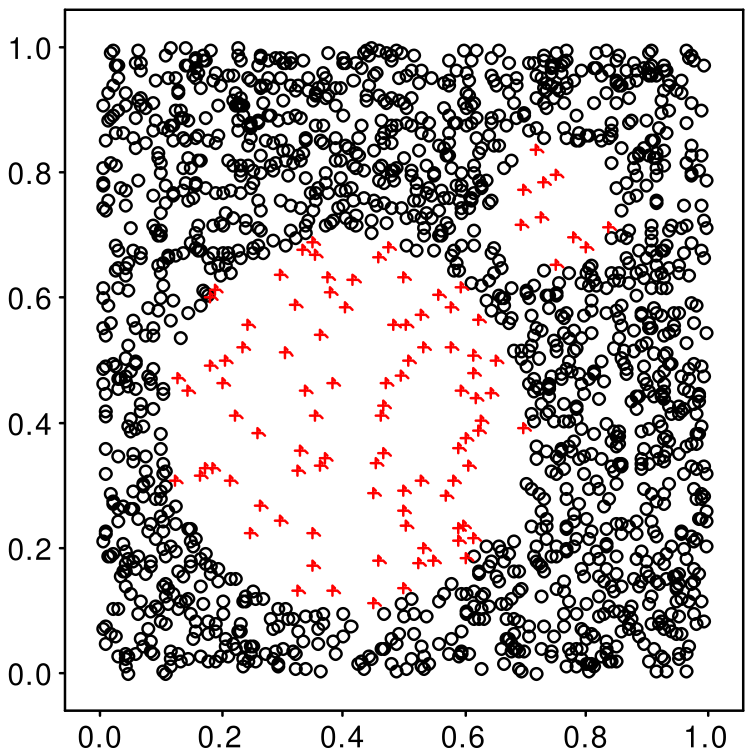
\includegraphics[width=\textwidth]{bl-smote-original.png}
        \caption{}
        \label{fig:blSMOTE-orig}
    \end{subfigure}
    \begin{subfigure}[b]{0.33\textwidth}
        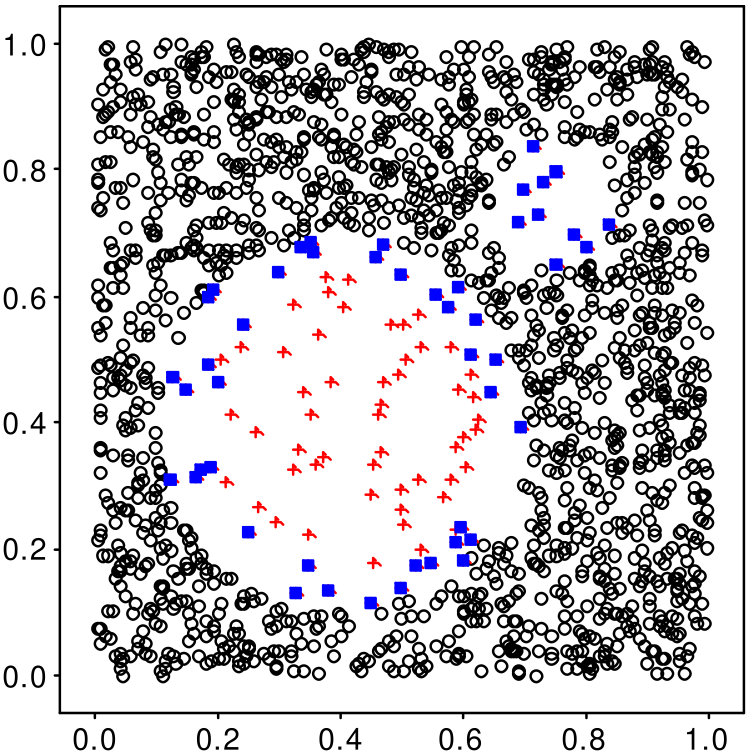
\includegraphics[width=\textwidth]{bl-smote-datos-borderline.png}
        \caption{}
        \label{fig:blSMOTE-border}
    \end{subfigure}
    \begin{subfigure}[b]{0.33\textwidth}
        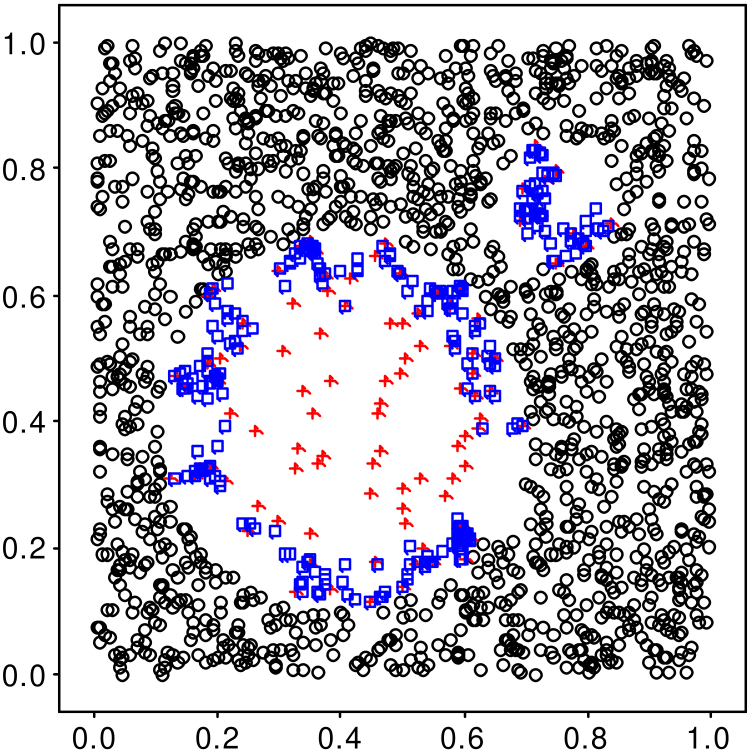
\includegraphics[width=\textwidth]{bl-smote-datos-sinteticos.png}
        \caption{}
        \label{fig:blSMOTE-sintetico}
    \end{subfigure}

    \caption{\ref{fig:blSMOTE-orig} Conjunto de datos original. \ref{fig:blSMOTE-border} datos que conforman el límite de la clase minoritaria (cuadros azules rellenos). \ref{fig:blSMOTE-sintetico} Nuevos datos generados de forma sintética dentro de los límites de la clase (cuadros azules no rellenos). Imagen obtenida de \cite{BL-SMOTE}.}
	 \label{fig:ejemploBL-SMOTE}

\end{figure}


\begin{figure}[H]
    \centering
	 \begin{subfigure}[b]{\textwidth}
		 \centering
		 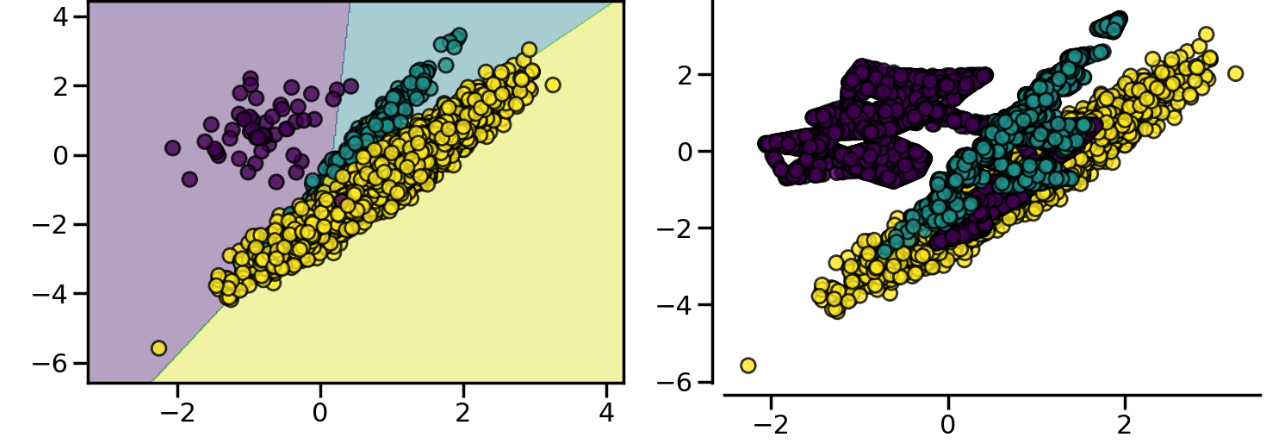
\includegraphics[width=0.8\textwidth]{resampling_smote.png}
		 \caption{A la izquierda bordes de las clases, y a la derecha sobremuestreo con SMOTE}
		 \label{fig:SMOTE-cmp}
	 \end{subfigure}

    \begin{subfigure}[b]{\textwidth}
		 \centering
		  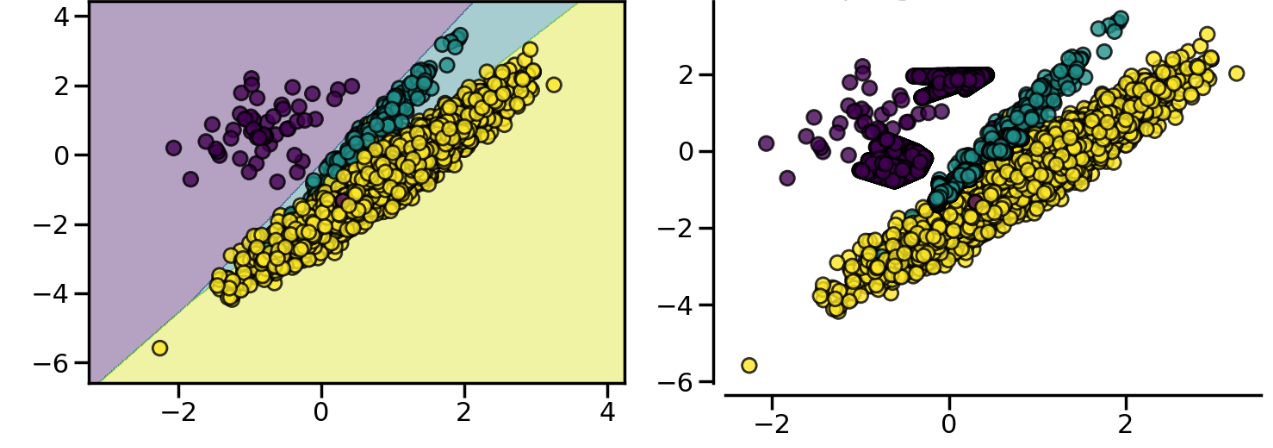
\includegraphics[width=0.8\textwidth]{resampling_blsmote.png}
        \caption{A la izquierda bordes de las clases, y a la derecha sobremuestreo con BorderlineSMOTE}
        \label{fig:BLSMOTE-cmp}
    \end{subfigure}

    \caption{Comparación de SMOTE y BorderlineSMOTE para un conjunto de datos generado aleatoriamente.}\label{fig:BLSMOTE-SMOTE}

\end{figure}

Esta claro que, como vemos en la figura \ref{fig:ejemploBL-SMOTE} y la figura \ref{fig:BLSMOTE-SMOTE}, esta técnica es mucho más versátil y conveniente que SMOTE.


\newpage

\subsection{Resultado tras el preprocesado}

% TODO: Ampliar esto cuando se aplique el preprocesado


\begin{table}[H]
\centering
\resizebox{\textwidth}{!}{%
\begin{tabular}{|c|c|c|c|}
\hline
\textbf{}                   & \textbf{Lateralidad izquierda} & \textbf{Lateralidad derecha} & \textbf{Conjunto completo} \\ \hline
\textbf{Original}           & 439                            & 453                          & 892                        \\ \hline
\textbf{Tras aplicar X} & 579                            & 592                          & 1182                       \\ \hline
\end{tabular}
}
\caption{Comparación del número de datos en el conjunto original y tras aplicar X.}\label{table:comparacion_orig_X}
\end{table}

Como vemos en las figuras \ref{fig:l0-over}, \ref{fig:l1-over} y \ref{fig:completo-over} hemos conseguido equilibrar la densidad de las etiquetas, reduciendo la densidad de las etiquetas con valores más altos, los más predominantes en el conjunto de datos, y creando nuevos datos sintéticos de etiquetas con menor valor. Además, como podemos ver en la tabla \ref{table:comparacion_orig_SMOGN}, aumentando el número de muestras, sin necesidad de que SMOGN haya aplicado submuestreo.
